\documentclass[12pt,letterpaper]{article}
\usepackage[utf8]{inputenc}
\usepackage[spanish, mexico]{babel}
\usepackage{amsmath}
\usepackage{amsfonts}
\usepackage{amssymb}
\usepackage{amsmath}
\usepackage[lmargin=3cm,rmargin=3cm,tmargin=3cm,bmargin=3cm]{geometry}

\usepackage{hyperref}
\usepackage{graphicx}
\usepackage{float}
\begin{document}

\title{Actividad 7: El espacio Fase}
\author{Luisa Fernanda Orci Fernandez.}
\date{10 de Marzo del 2016}

\maketitle

\section*{Espacio Fase}
El espacio fase, también conocido coo espacio fásico o diagrama de fases, cada punto de este espacio representa un estado del sistema físico y este espacio se caracteriza por cada uno de los momentos respectivos de cada "partícula". \\
El espacio fase es una herramienta de gran ayuda para estudiar sistemas dinámicos, tal es el caso del péndulo simple, un oscilador armńico simple o uno de Van de Pol, entre otros.

\section*{Actividad}
En esta actividad, como en las anteriores, seguimos trabajando con un péndulo pero la diferencia es que esta vez construiremos el Espacio fase del péndulo, este espacio representará cada una de las soluciones de un péndulo simple.\\
Para realizar esta actividad, se nos proporcionó un código ejemplo de $Lotka-Volterra$, (este se encuentra en $SciPy$ $CookBook$), el cual describía el comportamiento de una población de zorros y conejos, esto con fin de que nosotros lo modificaramos para representar el Espacio Fase de un péndulo simple con condiciones iniciales. Posteriormente recurrimos a $Matplotlib$ de $Python$ para gráficar el espacio fase.\\

El código final fue el siguiente:
\begin{verbatim}
#PAQUETES

import numpy as gatito
import matplotlib.pyplot as plt
from scipy.integrate import odeint

#CONSTANTES

g = 9.81
l = 1.0
b = 0.0 
c = g/l


#CONDICIONES INICIALES

X_f1 = gatito.array([-3*gatito.pi,gatito.pi])
X_f2 = gatito.array([-gatito.pi,gatito.pi])
t = gatito.linspace(0,20,300)



#ECUACION

def p (y, t, b, c):
    theta, omega = y
    dy_dt = [omega,-b*omega -c*gatito.sin(theta)]
    return dy_dt

#FORMATIUX

values  = gatito.linspace(-1.0,1.0,25)       
# position of X0 between X_f0 and X_f1
vcolors = plt.cm.winter_r(gatito.linspace(0.5, 1.0, len(values)))  
# colors for each trajectory

plt.figure(2)


for v, col in zip(values, vcolors):
    y0 = v * X_f1                              
    
 X = odeint(p, y0, t, args=(b,c))         
 plt.plot( X[:,0], X[:,1], lw=3.5*v, color=col, label='X0=(%.f, %.f)' 
 % ( y0[0], y0[1]) )

                              
for v, col in zip(values, vcolors):
 y1 = v * X_f2                           
 X1 = odeint(p, y1, t, args=(b,c))           
 plt.plot( X1[:,0], X1[:,1], lw=3.5*v, color=col, label='X0=(%.f, %.f)'
 % ( y1[0], y1[1]) )



#GRAFICA <3

plt.title('Trayectorias')
plt.xlabel('Angulo')
plt.ylabel('Velocidad Angular')
plt.grid()
plt.xlim(-2.0*gatito.pi,2.0*gatito.pi)
plt.ylim(-12,12)


plt.show()
\end{verbatim}

y la gráfica resultante fue la siguiente: 
\begin{center}

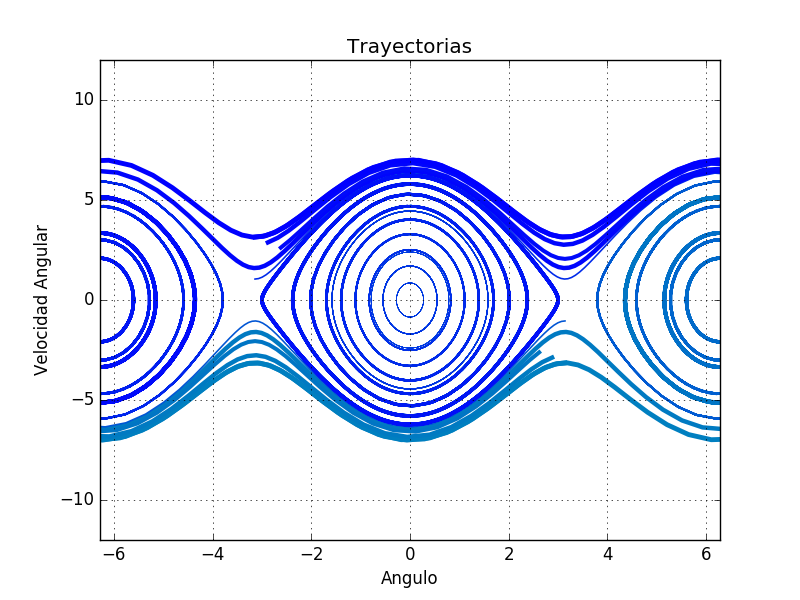
\includegraphics[scale=0.6]{actividad7.png}

\end{center}

 
\section*{Conclusiones}
Esta actividad, como todas las anteriores, se me hizo de gran interes, no solo por que ahora sabemos como graficar espacios fase en $Python$, si no por que en un futuro será de gran ayuda.

\begin{thebibliography}{widestlabel}
      \bibitem{1} Wikipedia, \emph{Espacio Fásico}, (2016, 10 de Marzo).Desde: \url{https://es.wikipedia.org/wiki/Espacio_f\%C3\%A1sico}
\end{thebibliography}


\end{document}